
\chapter{Motion along a Straight Line}

\section{Discussion Questions}

% 2.1
\discussion{Speed.  Velocity has a direction as well as a magnitude.}

% 2.2
\discussion{Since the dots appear to be increasing by what appears a multiple of the previous distance I would say it is graph (d).}

% 2.3
\discussion{Yes, if the velocity and acceleration have ``different signs''.  This is because the velocity is ``slowing down'' and will eventually reach zero, then start ``increasing again''.  You can also look at the formula for velocity with constant acceleration to see why.  It cannot reverse twice though as a straight line cannot pass through the x-axis twice.}

% 2.4
\discussion{Either when the velocity is constant or special cases when the acceleration changes direction and after a period of time the average velocity will match the instantaneous velocity.}

% 2.5
\discussion{ (b) Yes.  When the velocity and acceleration are in ``opposite directions''.  Yes, if they both point in the ``same direction''.}

% 2.6
\discussion{Constant acceleration.  Anytime you start from 0 speed and accelerate then end up at 0 speed will the speed equal the magnitude of the velocity at some point.}

% 2.7
\discussion{Average velocities are the same but in opposite directions.}

% 2.8
\discussion{You could argue that you would be able to ticket all parked cars that people who speed pass by.}

% 2.9
% This question is no very clear.  I assume they mean instantaneous velocity when they say velocity.
\discussion{No, because displacement is 0, $\Delta{x}$ = zero, then by definition the average velocity is 0.  For the second yes;  $x =sin(t)$, then $y=cos(t)$.  When t = 0 displacement is 0 but velocity is 1.}

% 2.10
\discussion{Yes. If you assume the object is already moving and there is no acceleration then the object will keep moving.}

% 2.11
\discussion{180km/hr * 1h/60m * 1m = 3km. 6.0 seconds is 1/10th of a minute, so 1/10th of 3km, 0.3km}

% 2.12
\discussion{360km/hr, since this is linear half the time means twice the speed.}

% 2.13
\discussion{(a) one being a straight line and the other being a parabola going throught the two points.  (b) Average V is $\delta{x}/\delta{t}$ so same for both.}

% 2.14
\discussion{No.  Imagine the top half of a circle starting a 0~\si{\meter/\second} and ending with 0~\si{\meter/\second}, the average would be 0, which it obviously isn't.}

% 2.15
\discussion{Thrown.  The distance travelled to go from 0 to the starting speed is more than the distance from your hand to the top.  If you calculate the acceleration you can see that in your hand is higher.}

% 2.16
\discussion{Your friend will beat you, it takes you $\frac{21}{20}~\si{\hour}$ and your friend $\frac{3}{5}~\si{\hour}$.}

% 2.17
\discussion{-9.8\si{\meter/\second^2}, it starts at that value but decreases over time.}

% 2.18
\discussion{The elevator.}

% 2.19
\discussion{(a) Same speed (b) Ball thrown down (c) Same (d) Ball thrown up }

% 2.20
\discussion{Less than 4~\si{\meter/\second}}

% 2.21
\discussion{Velocity is 0, and it is changing.  This change is the acceleration.}

% 2.22
\discussion{$\sqrt(3)T$}

\section{Exercises}

\subsection*{Displacement, Time, and Average Velocities}

% 2.1
\exercise{\distance{32.9}}

% 2.2
\exercise{
(a) \velocity{-0.00476} \\
(b) \velocity{0}
}

% 2.3
\exercise{1.38 hours longer}

% 2.4
\exercise{
(a) \velocity{4.4} \\
(b) \velocity{-7.3}}

% 2.5
\exercise{
(a) \velocity{0.28} \\
(b) \velocity{1.25}}

% 2.6
\exercise{
(a) \velocity{2.74} \\
(b) \velocity{4.94} \\
(c) \velocity{7.40}
}

\subsection*{Instantaneous Velocity}

% 2.7
\exercise{
(a) \velocity{41} \\
(b) v(0) = \velocity{21.8}, v(10) = \velocity{27}
}

% 2.8
\exercise{\velocity{3.62}}

% 2.9
\exercise{(a) $\frac{7}{3}$~\si{\meter/\second}, same for both (b) $V_{avg} = \frac{1}{3}$~\si{\meter/\second} $Speed_{avg} = \frac{7}{3}$~\si{\meter/\second} }

% 2.10
\exercise{(a) \rom{4} (b) \rom{1} (c) \rom{5} (d) \rom{2} (e) none }

% 2.11
\exercise{
A: \velocity{$\frac{20}{3}$} \\
B: \velocity{$\frac{20}{3}$} \\
C: \velocity{$0$} \\
D: \velocity{$-40$}
}

\subsection*{Average and Instantaneous Acceleration}

% 2.12
\exercise{
(a) (i) \acceleration{6} (ii) \acceleration{-6} (iii) \acceleration{0} (iv) \acceleration{0} \\
(b) \acceleration{0} and \acceleration{-6}
}

\begin{figure}[!ht]
    \centering
    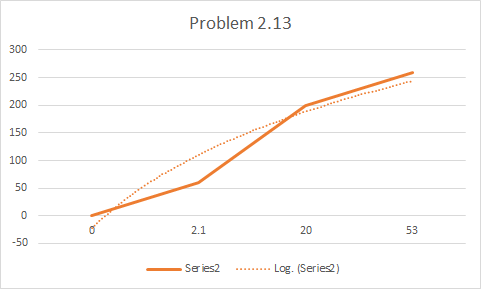
\includegraphics[scale=0.5]{mechanics/chapter2/problem2.13Speed.png}
    \caption{Problem 2.13}
    \label{fig:Problem2.13}
\end{figure}


% 2.13
\exercise{
(a) \Fig{fig:Problem2.13} \\
(b) (i) $\acceleration{28.6}$ (ii) $\acceleration{7.82}$ (iii) $\acceleration{1.82}$
}

% 2.14
\exercise{\acceleration{6.93}}

\begin{figure}[ht!]
    \begin{minipage}{.5\linewidth}
    \centering
    \subfloat[Position]{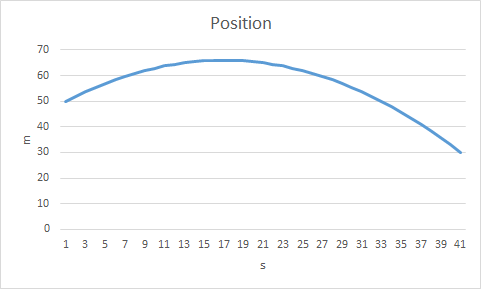
\includegraphics[scale=0.45]{mechanics/chapter2/problem2.15Position.png}\label{fig:Problem2.15Position}}
    \end{minipage}%
    \begin{minipage}{.5\linewidth}
    \centering
    \subfloat[Velocity]{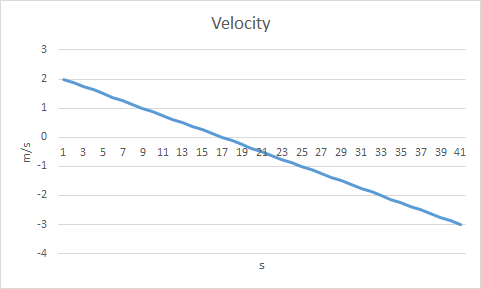
\includegraphics[scale=0.45]{mechanics/chapter2/problem2.15Velocity.png}\label{fig:Problem2.15Velocity}}
    \end{minipage}\par\medskip
    \centering
    \subfloat[Acceleration]{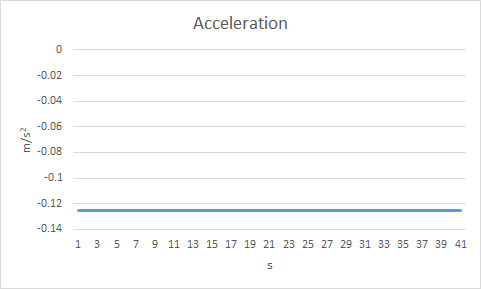
\includegraphics[scale=0.45]{mechanics/chapter2/problem2.15Acceleration.png}\label{fig:Problem2.15Acceleration}}

    \caption{Problem 2.15}
    \label{fig:Problem2.15}
\end{figure}

% 2.15
\exercise{(a) 2.00~\si{\centi\meter/\second} 50.0~\si{\centi\meter} 0.125~\si{\centi\meter/\second^2} \\
(b) \seconds{16} \\
(c) \seconds{32} \\
(d) \seconds{-13.9} and \seconds{45.9} \\
(e) \Fig{fig:Problem2.15}
}

% 2.16
\exercise{
(a) mag: \acceleration{0.963} sign: positive dir: right \\
(b) mag: \acceleration{0.963} sign: negative dir: left  \\
(c) mag: \acceleration{2.83} sign: negative dir: left
}

\begin{figure}[ht!]
    \begin{minipage}{.5\linewidth}
        \centering
        \subfloat[Position]{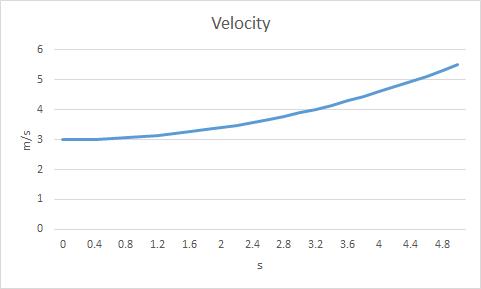
\includegraphics[scale=0.45]{mechanics/chapter2/problem2.17Velocity.png}\label{fig:Problem2.17Velocity}}
    \end{minipage}%
    \begin{minipage}{.5\linewidth}
        \centering
        \subfloat[Velocity]{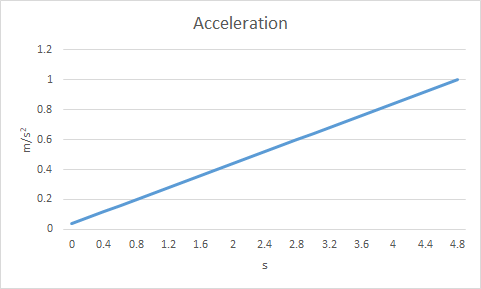
\includegraphics[scale=0.45]{mechanics/chapter2/problem2.17Acceleration.png}\label{fig:Problem2.17Acceleration}}
    \end{minipage}\par\medskip

    \caption{Problem 2.17}
    \label{fig:Problem2.17}
\end{figure}

% 2.17
\exercise{ 
(a) $0.5~\acceleration$ (b) \Fig{fig:Problem2.17}
}

\begin{figure}[ht!]
    \begin{minipage}{.5\linewidth}
    \centering
    \subfloat[Position]{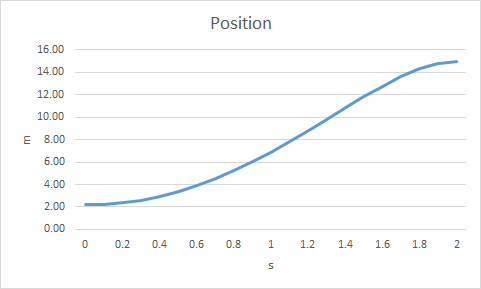
\includegraphics[scale=0.45]{mechanics/chapter2/problem2.18Position.png}\label{fig:Problem2.18Position}}
    \end{minipage}%
    \begin{minipage}{.5\linewidth}
    \centering
    \subfloat[Velocity]{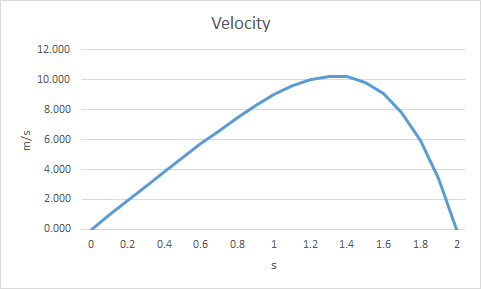
\includegraphics[scale=0.45]{mechanics/chapter2/problem2.18Velocity.png}\label{fig:Problem2.18Velocity}}
    \end{minipage}\par\medskip
    \centering
    \subfloat[Acceleration]{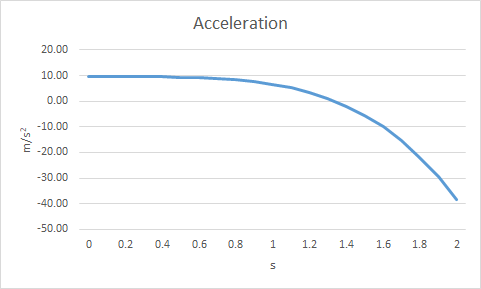
\includegraphics[scale=0.45]{mechanics/chapter2/problem2.18Acceleration.png}\label{fig:Problem2.18Acceleration}}

    \caption{Problem 2.18}
    \label{fig:Problem2.18}
\end{figure}

% 2.18
\exercise{
(a) t = 0 x = \distance{2.17}, t=+2 x = \distance{15}, t=-2 x = \distance{15} \\
(b) \Fig{fig:Problem2.18}
}

\subsection*{Motion with constant Acceleration}

% 2.19
\exercise{
(a) \velocity{5.40} \\
(b) \acceleration{1.36}
}

% 2.20
\exercise{
(a) Yes \\
(b) \velocity{245}
}

% 2.21
\exercise{\acceleration{736}}

% 2.22
\exercise{
(a) \acceleration{2500} \\
(b) \distance{1.06}
}

% 2.23
\exercise{\distance{1.55}}

% 2.24
\exercise{
(a) \seconds{33.8} \\
(b) \distance{662}
}

% 2.25
\exercise{\distance{0.38}}

% 2.26
\exercise{
(a) \acceleration{-39} \\
(b) \seconds{0.018}
}

% 2.27
\exercise{
(a) \acceleration{3.13e6} \\
(b) \seconds{0.016} \\
(c) No
}

% 2.28
\exercise{
(a) \velocity{1.4} \\
(b) \seconds{13} \\
(c) \distance{234}
}

% 2.29
\exercise{
(a) (i) 7.11e4\si{\kilo\meter/\hour^2} (ii) 9.84e4\si{\kilo\meter/\hour^2} \\
(b) (i) 0.18~\si{\kilo\meter} (ii) 13~\si{\kilo\meter}
}

% 2.30
\exercise{
(a) 1.7\si{\centi\meter/\second} \\
(b) 1.4\si{\centi\meter/\second} \\
(c) TODO: Take picture
}

% 2.31
\exercise{
(a) \acceleration{7.5}, \acceleration{12.5} \\
(b) \distance{400}, \distance{195}, \distance{285}
}

% 2.32
\exercise{
TODO: Do and take picture of resulting graphs.
}

% 2.33
\exercise{
$V_f$ = \velocity{2.68}
}

% 2.34
\exercise{
(a) \distance{246} \\
(b) \velocity{41.1} \\
(c) TODO: Take picture \\
(d) TODO: Take picture
}

\subsection*{Freely Falling Bodies}

% 2.35
\exercise{
$v = \sqrt{2g\Delta{x}}$, $t = 2\Delta{x}/(V_0+V_f)$ \\
(a) \velocity{4.6} \\
(b) \seconds{0.116}
}

% 2.36
\exercise{
   (a) \velocity{32.4} \\
   (b) \seconds{1.47}
}

% 2.37
\exercise{
    \seconds{1.65}
}

% 2.38
\exercise{
	(a) \velocity{4.11} \\
	(b) \seconds{0.468}
}

% 2.39
\exercise{
	(a) \distance{26.0} \\
	(b) \velocity{13.9} \\
	(c) TODO
}

% 2.40
\exercise{
	\velocity{-4.1}
}

% 2.41
\exercise{
	(a) $t = \sqrt{2\Delta{X}/a}$ \\
	(b) \seconds{0.059}
}

% 2.42
\exercise{
	(a) \distance{17.7} \\
	(b) \velocity{18.6} \\
	(c) TODO
}

% 2.43
\exercise{
	(a) \distance{678} \\
	(b) \seconds{11} \\
	(c) TODO
}

% 2.44
\exercise{
	(a) x(0.155) = \distance{0.66}, x(1.20) = \distance{-1.06} \\
	(b) \seconds{23} \\
	(c) \velocity{-220} \\
	(d) \distance{41m} \\
	(e) TODO
}

% 2.45
\exercise{
	(a) \acceleration{250} \\
	(b) 25.5 \\
	(c) \distance{21} \\
	(d) No, only 21g
}

% 2.46
\exercise{
	(a) \velocity{17.1} \\
	(b) \distance{14.9} \\
	(c) \velocity{0} \\
	(d) \acceleration{-9.8} \\
	(e) TODO
}

% 2.47
\exercise{
	\velocity{0.0868}
}

% 2.48
\exercise{
	(a) \seconds{2.03} \\
	(b) \seconds{6.21} \\
	(c) \seconds{0} and \seconds{8.24} \\
	(d) \seconds{4.12} \\
	(e) All are \acceleration{-9.8} \\
	(f) TODO
}

% 2.49
\exercise{
	$V_f = \velocity{17.8}$
}

% 2.50
\exercise{
	\distance{47.3}
}

% 2.51
\exercise{
	(a) \distance{500} \\
	(b) \velocity{103} 
}

% 2.52
\exercise{
	(a) \velocity{689} \\
	(b) \distance{11.5} \\
	(c) TODO
}

% 2.53
\exercise{
	(a) $a(t) = At - Bt^2$, $v(t) = \frac{At^2}{2} - \frac{Bt^3}{3}$, $x(t) = \frac{At^3}{6} - \frac{12}{Bt^4}$ \\ 
	(b)\velocity{39.1}
}

% 2.54
\exercise{
	REDO
}

\section{Problems}

\section{Challenge Problems}